\documentclass[12pt]{article}
\usepackage[utf8]{inputenc}
\usepackage{upquote}
\usepackage[margin=20mm]{geometry} 
\usepackage{amsmath,amsthm,amssymb}
\usepackage{graphicx}
\usepackage{listings}
\newenvironment{statement}[2][Statement]{\begin{trivlist}
\item[\hskip \labelsep {\bfseries #1}\hskip \labelsep {\bfseries #2.}]}{\end{trivlist}}
\usepackage{xcolor}

\usepackage{subfigure}


% Listings package for code rendering (No external dependencies)
\usepackage{listings}  
\usepackage{xcolor}   % Color support
\usepackage{tcolorbox} % Box for better appearance

% Define custom colors for code highlighting
\definecolor{codegreen}{rgb}{0,0.6,0}
\definecolor{codegray}{rgb}{0.5,0.5,0.5}
\definecolor{codepurple}{rgb}{0.58,0,0.82}
\definecolor{backcolour}{rgb}{0.95,0.95,0.92}


\lstset{frame=tb,
    language=Python,
    backgroundcolor=\color{backcolour},   
    commentstyle=\color{codegreen},
    keywordstyle=\color{magenta},
    numberstyle=\tiny\color{codegray},
    stringstyle=\color{codepurple},
    basicstyle=\ttfamily\footnotesize,
    breakatwhitespace=false,         
    breaklines=true,                 
    keepspaces=true,                 
    numbers=left,       
    numbersep=5pt,                  
    showspaces=false,                
    showstringspaces=false,
    showtabs=false,                  
    tabsize=2,
}





\title{Assignment 6}


\author{Author \\
 Wanjing Hu / fng685@alumni.ku.dk  \\
 Shuangcheng Jia / bkg713@alumni.ku.dk/   \\
 Zhigao Yan / sxd343@alumni.ku.dk  \\
} 

\begin{document}
\maketitle

\section{Transformations on images - Translation}
%zhigao
\subsection{}
Translating one pixel to the right means that the value of each point (x,y) in the new image should be taken from the position of one pixel to the left of the original image.

The mathematical expression can be:
 \[
\tilde{I}(x,y) = I\bigl(x - 1,\, y\bigr).
\]
\subsection{}

In the homogeneous coordinate, the transformation matrix for a 1-pixel translation to the right is:
\[
M = 
\begin{pmatrix}
1 & 0 & 1 \\
0 & 1 & 0 \\
0 & 0 & 1
\end{pmatrix}
\]

\[
\begin{pmatrix}
x' \\[6pt]
y' \\[6pt]
1
\end{pmatrix}
=
M
\cdot
\begin{pmatrix}
x \\[6pt]
y \\[6pt]
1
\end{pmatrix}
\quad\Longrightarrow\quad
\tilde{I}(x', y') = I(x, y)
\]
\subsection{}
If we use convolution:
\[
K = 
\begin{bmatrix}
0 & 0 & 0 \\
0 & 0 & 1 \\
0 & 0 & 0
\end{bmatrix}
\]
For Correlation:
\[
K = 
\begin{bmatrix}
0 & 0 & 0 \\
1 & 0 & 0 \\
0 & 0 & 0
\end{bmatrix}
\]
\subsection{}
Image size is 17*17, square size is 5*5.
\begin{figure}[h]
    \centering
    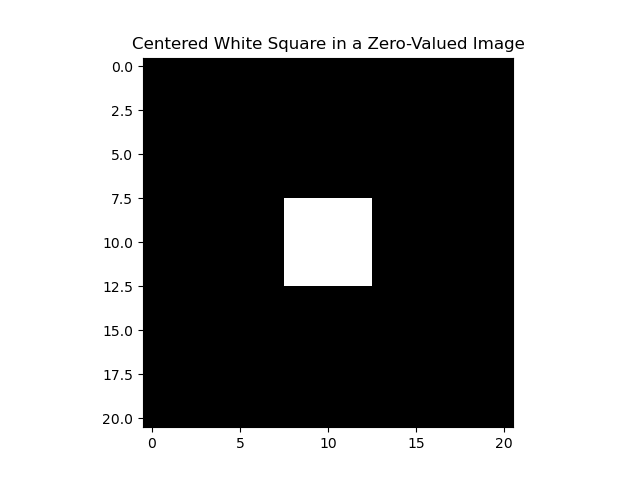
\includegraphics[width=0.6\textwidth]{pics/a6_1.4.png} 
    \caption{Zero-Valued Image}
\end{figure}
\subsection{}
\begin{figure}[ht]
    \centering
    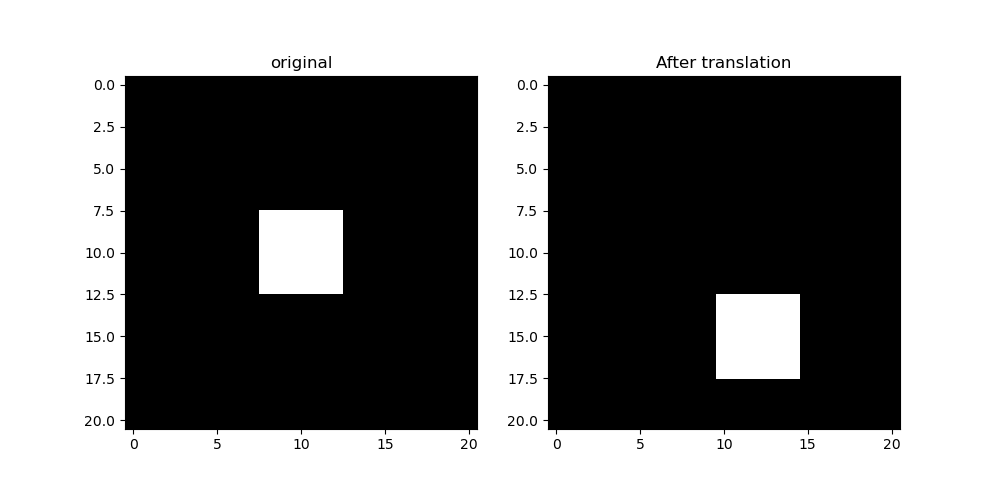
\includegraphics[width=0.6\textwidth]{pics/a6_1.5.png} 
    \caption{Zero-Valued Image after translation}
\end{figure}
I showed the original image as well as the image that was first translated 2 pixels to the right and then 5 pixels down.
\begin{lstlisting}
def translate_image(image, dx=0, dy=0, boundary='symm'):
    
    # Generate horizontal translation kernels
    kernel_x = np.zeros((1, 2*abs(dx)+1))
    kernel_x[0, abs(dx) + dx] = 1  
    print(kernel_x)
    
    # Generate vertical translation kernels
    kernel_y = np.zeros((2*abs(dy)+1, 1))
    kernel_y[abs(dy) + dy, 0] = 1
    print(kernel_y)
    
    # Translation in both directions
    shifted = convolve2d(image, kernel_x, mode='same', boundary=boundary)
    shifted = convolve2d(shifted, kernel_y, mode='same', boundary=boundary)
    return shifted
\end{lstlisting}
The code is to first generate two translational kernels and then convolve the images separately.
Scipy provides three boundary conditions, which are:
'fill': pad input arrays with fillvalue.
'wrap': circular boundary conditions.
'symm': symmetrical boundary conditions.
\subsection{}
\begin{lstlisting}
    def translate_image_homogeneous(image, tx, ty):
    rows, cols = image.shape
    # Create target image (initialised to 0)
    translated = np.zeros_like(image)
    
    # homogeneous coordinate
    T = np.array([[1, 0, tx],
                  [0, 1, ty],
                  [0, 0, 1]])
    
    for i in range(rows):
        for j in range(cols):
            # Find the inverse matrix of homogeneous coordinate and multiply the transformed coordinates.
            x, y, _ = np.linalg.inv(T) @ [i, j, 1]
            # nearest neighbor interpolation
            x_round = int(round(x))
            y_round = int(round(y))
            # Check that the image limit is not exceeded.
            if 0 <= x_round < rows and 0 <= y_round < cols:
                translated[i, j] = image[x_round, y_round]
    
    return translated
\end{lstlisting}
First I would initialise an image the same size as the original and set all the initial values to 0. Then construct homogeneous coordinate and multiply them according to the eq 1.2. Then get the closest coordinates for interpolation, and return an image.
\begin{figure}[ht]
    \centering
    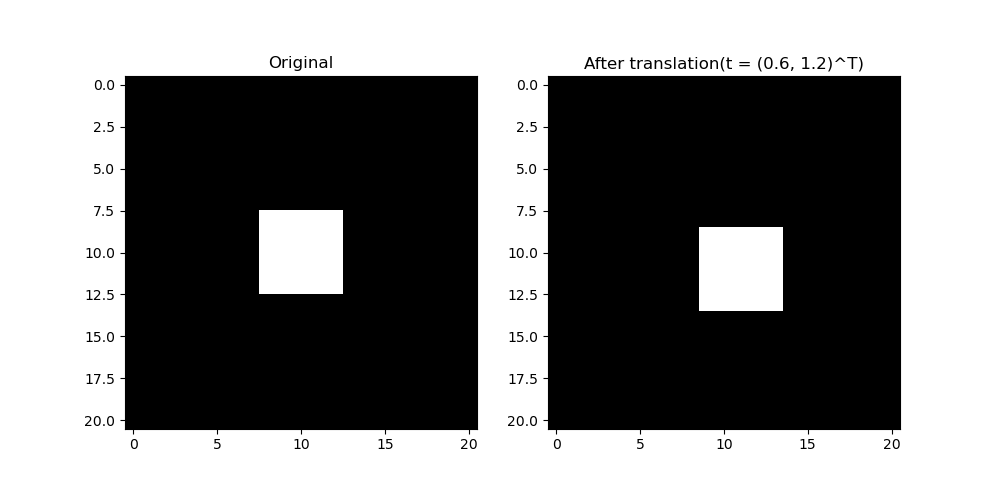
\includegraphics[width=0.6\textwidth]{pics/a6_1.6.png} 
    \caption{Non-integer translations}
\end{figure}


The image on the left is the image that was first shifted 0.6 to the right and then 1.2 down.
\newpage
\subsection{}
\begin{lstlisting}
    def fourier_translate(image, tx, ty):

    # Calculate the frequencies separately and then combine the frequency grids
    rows, cols = image.shape
    u = np.fft.fftfreq(cols)  
    v = np.fft.fftfreq(rows)  
    U, V = np.meshgrid(u, v)  

    # Calculate the Fourier transform
    F = fft2(image)
    
    # Fourier transform translation equation.
    phase_shift = np.exp(-2j * np.pi * (tx * U + ty * V))

    
    F_translated = F * phase_shift

    # Inverse Fourier transform back to the spatial domain
    translated_image = np.real(ifft2(F_translated))

    return translated_image
\end{lstlisting}

\begin{figure}[ht]
    \centering
    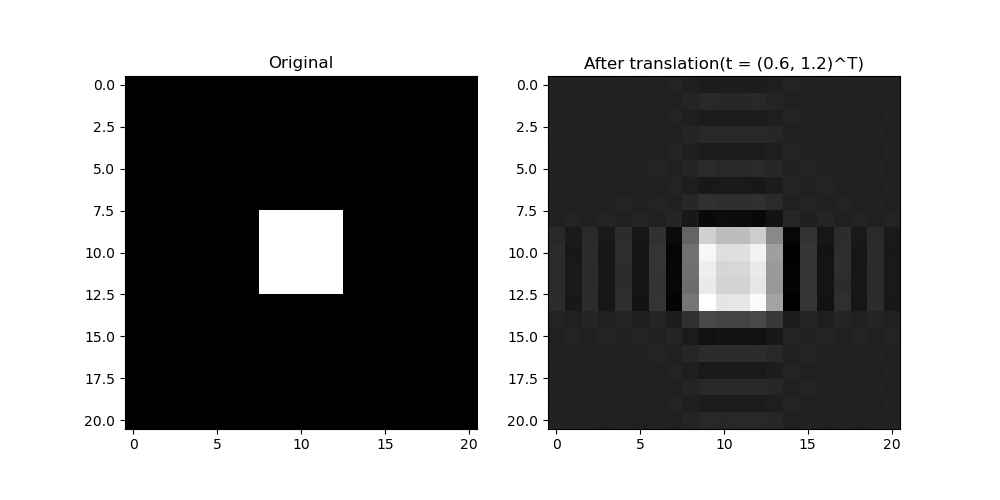
\includegraphics[width=0.6\textwidth]{pics/a6_1.7.png} 
    \caption{Fourier transform translation.}
\end{figure}
My code is built based on the following equation:
\[
f(x - a, y - b) \quad \xrightarrow{\mathcal{F}} \quad F(u,v) e^{-i 2\pi (ua + vb)}
\]
It seems to me that this Fourier transform translation method cannot cope with non-integer numbers. As we can see from the image, there is a blurring of the image after the translation, which proves that the pixels are not in the correct position.

\subsection{}
\begin{figure}[ht]
    \centering
    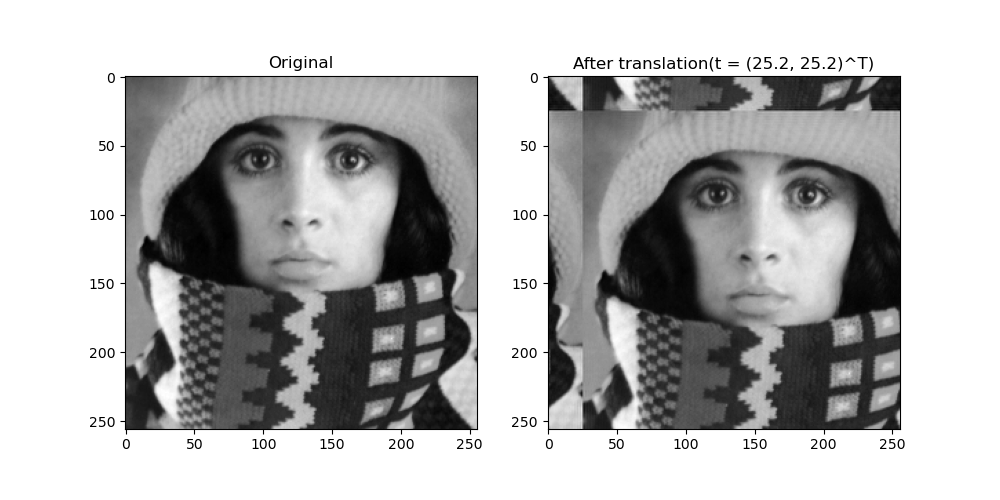
\includegraphics[width=0.6\textwidth]{pics/a6_1.8.png} 
    \caption{Fourier transform translation for real image}
\end{figure}
The method of the Fourier transform can be used for non-integer translations. I applied it to a real image and found that the blurring effect was not too noticeable, and that the out-of-range image was added to the edges after the translation.
I'm guessing that the white square pictures have sharp edges, so that causes a loss of precision in the high frequency components corresponding to the edges, whereas the normal pictures have relatively smooth edges, so the effect is small.
\section{Feature detection and image transforms}
%wanjing
\textbf{Step1 Preprocess}
We apply Gaussian Blur to reduce noise and smooth out variations. We choose a kernel sized (5,5).
\begin{lstlisting}
image = io.imread(image_path, as_gray=True)
blurred_image = cv2.GaussianBlur(image, (5, 5), 0)  # Kernel size (5,5)
\end{lstlisting}


\textbf{Step2 Corner Detection}
We use Harris Corner Detector to identify key points in the image where intensity changes sharply. The method is set to k to use the Harris response formula, and sigma=1 for standard deviation for Gaussian smoothing. The min distance is set 10 to ensure the detected corners are at least 10 pixels apart. The threshold rel is set to 0.01 to filter weak corner responses.
\begin{lstlisting}
corners_response = corner_harris(blurred_image, method='k', k=0.04, sigma=1)
corners = corner_peaks(corners_response, min_distance=10, threshold_rel=0.01)
\end{lstlisting}

\textbf{Step3 Corner Selection}
The detected points are converted to (x,y) format for processing, and we apply a sorting heuristic  to identify the four primary corners of the label: top-left, top-right, bottom-left, and bottom-right.
\begin{lstlisting}
# Convert (row, col) to (x, y)
corners = np.fliplr(corners)   
# Sort by x, then y
sorted_corners = sorted(corners, key=lambda x: (x[0], x[1])) 
top_left, top_right = sorted_corners[0], sorted_corners[-1]
bottom_left, bottom_right = sorted_corners[1], sorted_corners[-2]
\end{lstlisting}

\textbf{Step4 Estimating Rotation Angle}
The required rotation angle is computed using the atan2 function based on the x-y difference between the top-left and top-right corners. This gives the required rotation angle in degrees, valued -57.28.

\begin{lstlisting}
delta_x = top_right[0] - top_left[0]
delta_y = top_right[1] - top_left[1]
angle = np.arctan2(delta_y, delta_x) * (180.0 / np.pi)  # Convert to degrees
\end{lstlisting}

\textbf{Step5 Image Rotation and Visualization}
Here we plot the detected corners overlayed on the original image. And we display the final rotated image.

The parameter resize=True ensures the entire image remains within frame after rotation. 

Our final result is issued in Figure~\ref{rot}.
\begin{lstlisting}
rotated_image = transform.rotate(image, -angle, resize=True)

fig, ax = plt.subplots(1, 2, figsize=(12, 6))
ax[0].imshow(image, cmap="gray")
ax[0].scatter(corners[:, 0], corners[:, 1], color="red", s=20, label="Corners")
ax[0].set_title("Detected Corners")
ax[0].legend()

ax[1].imshow(rotated_image, cmap="gray")
ax[1].set_title(f"Rotated Image by {-angle:.2f} Degrees")

plt.show()
\end{lstlisting}

% describe the essential steps in your solution including relevant code snippets.

% specify all relevant parameters in the report

% detected label corner points overlayed on top of the image 

% the resulting rotated image and state your estimated rotation angle.

\begin{figure}[h]
    \centering
    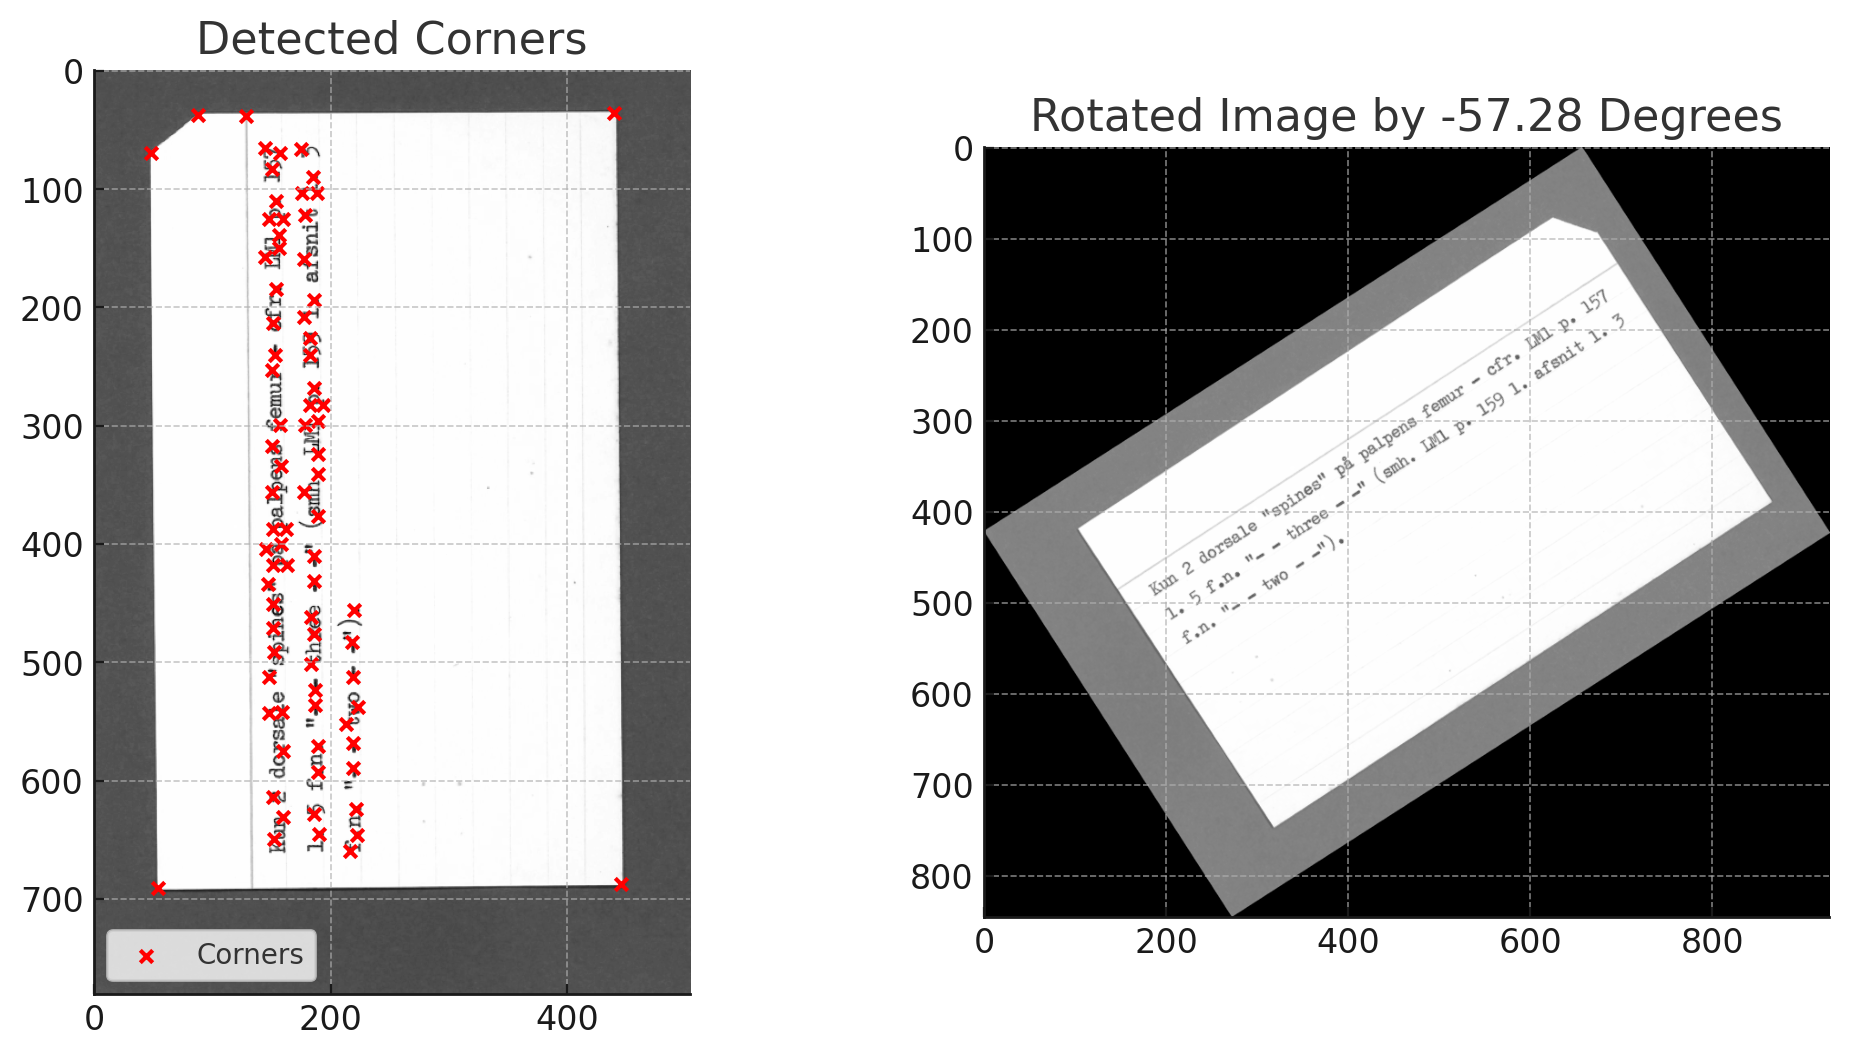
\includegraphics[width=0.8\textwidth]{pics/a6-2.1.png} 
    \caption{Estimated Rotation Angle: -57.28 degrees}
    \label{rot}
\end{figure}


\section{Features, filter banks and texture}
%shuangcheng
    \subsection{}
At the beginning, construct a filter bank using Gaussian derivative filters of first, second, and third orders at multiple scales. These filters are generated based on scale-normalized derivatives of the Gaussian function, ensuring appropriate sensitivity to structures of different sizes. The input image is loaded in grayscale and convolved with these filters in both the horizontal and vertical directions to extract features related to edges and textures.
\begin{figure}[h]
    \centering
    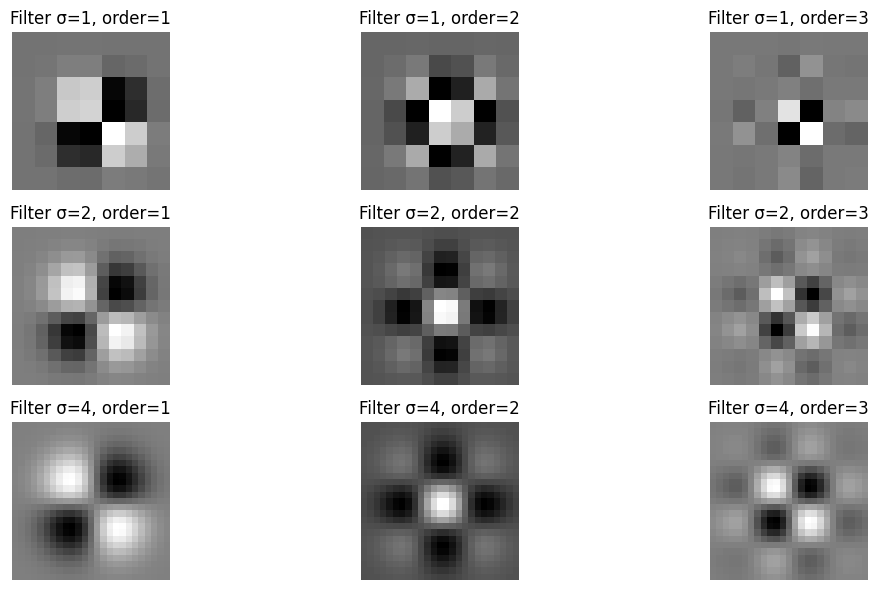
\includegraphics[width=0.9\textwidth]{pics/a6-3.1-1.png}
    \caption{Visualizations of Filters and Filter Responses}
    \label{3.1-1}
\end{figure}

\begin{figure}[h]
    \centering
    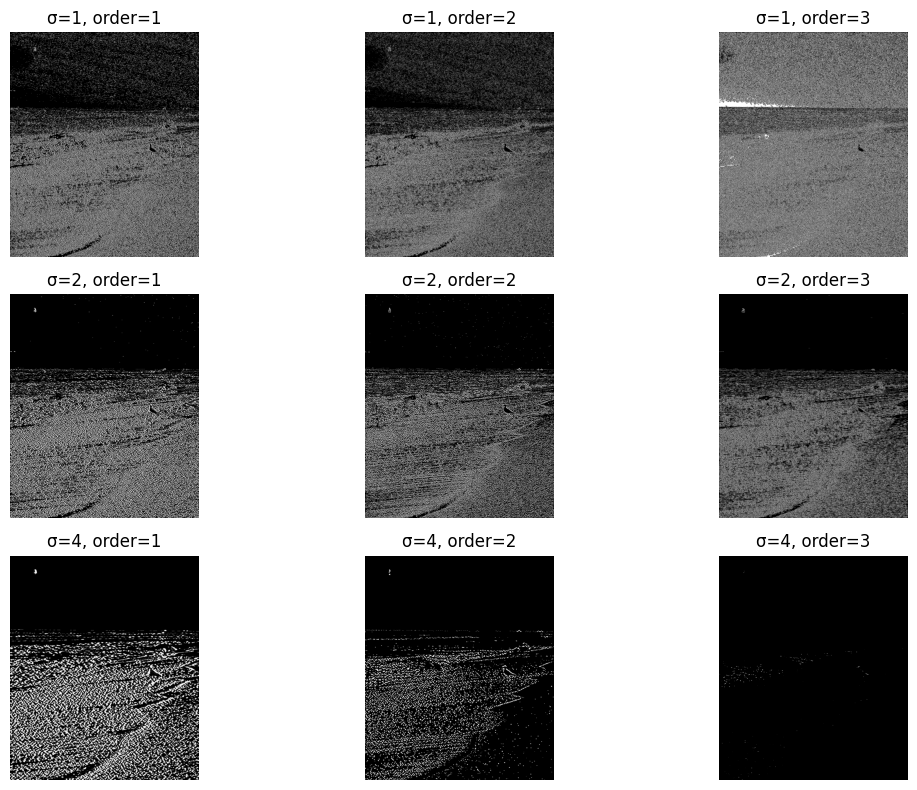
\includegraphics[width=0.9\textwidth]{pics/a6_3.1.png}
    \caption{Visualizations of Filters and Filter Responses}
    \label{3.1}
\end{figure}

The filtering results shown in Fig \ref{3.1} and Fig \ref{3.1-1} highlight different structural details, with lower-order derivatives enhancing edges and higher-order derivatives capturing more intricate variations. Finally, the filtered images are visualized to analyze the responses at different scales and derivative orders, providing insight into how textures and features evolve across scales.

\subsection{}
Firstly, extract small patches of size 8×8 from the grayscale image, using either a custom patch extraction function or the extract\_patches\_2d function from sklearn. These patches are then vectorized and used as input to Principal Component Analysis (PCA), which identifies the most significant patterns in the image by computing the principal components. The top principal components serve as learned filters, representing dominant edge and texture patterns in the data. These PCA-derived filters are then applied to the original image via convolution to generate filtered images, highlighting different structural features. The results are visualized by displaying the learned filters in Fig \ref{3.2-1} and the corresponding filter responses in Fig \ref{3.2-2}.

\begin{figure}[h]
    \centering
    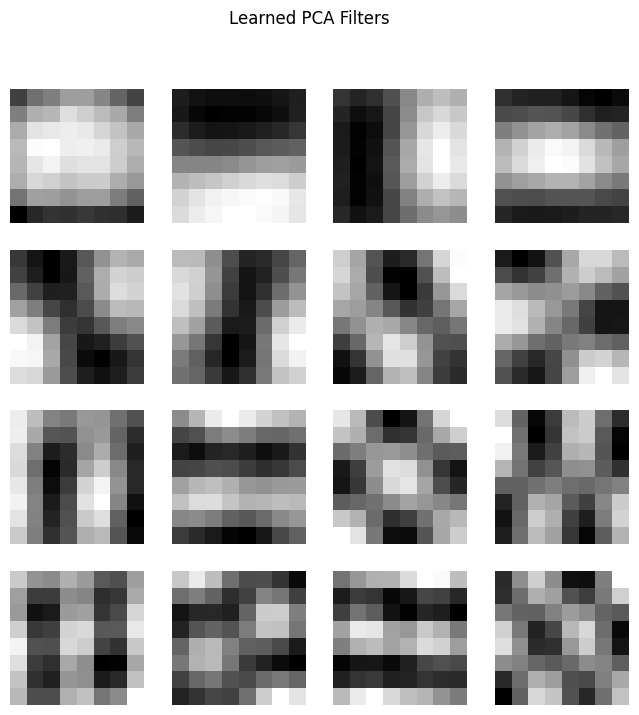
\includegraphics[width=0.4\textwidth]{pics/a6-3.2-1.png}
    \caption{Visualizations of Filters}
    \label{3.2-1}
\end{figure}

\begin{figure}[h]
    \centering
    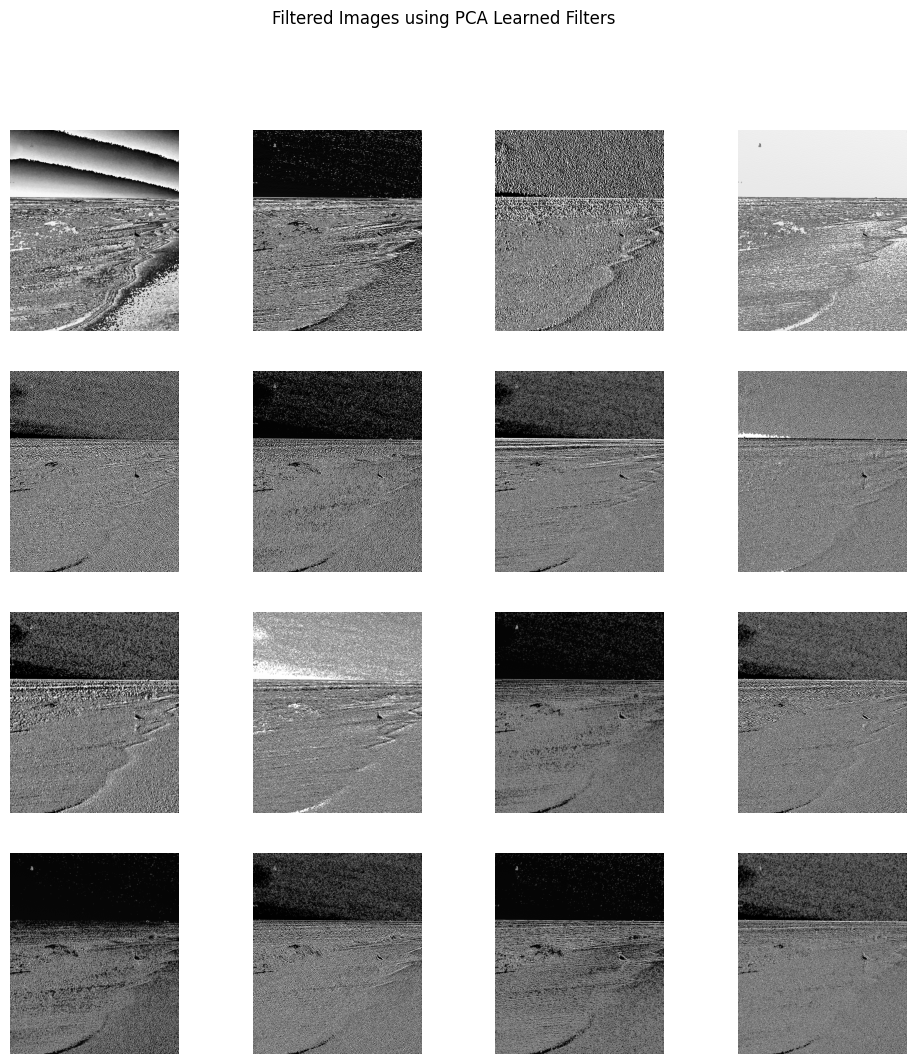
\includegraphics[width=0.6\textwidth]{pics/a6-3.2-2.png}
    \caption{Visualizations of Filter Responses}
    \label{3.2-2}
\end{figure}

The N-Jet filter bank is manually designed using Gaussian derivatives, while PCA-based filters are data-driven, adapting to the statistical structure of the image. N-Jet filters capture edges at multiple scales in a structured way, whereas PCA filters highlight dominant patterns specific to the image. PCA may discover more adaptive features but is less interpretable than predefined Gaussian derivatives.

\subsection{}
First, we briefly give some introduction to the basic steps of how we realize these two segmentation processes:

For PCA-Based Segmentation, the image is divided into small non-overlapping patches, which are flattened into feature vectors. PCA is applied to reduce dimensionality, preserving key information while improving clustering efficiency. The features are then normalized, and K-Means clustering is used to segment the image. The cluster labels are mapped back to reconstruct the segmented image, with a median blur applied to refine the boundaries.

For N-Jet-Based Segmentation with Rotation Invariance and PCA, multi-scale N-Jet filters extract edge and texture features from the image. To ensure rotation invariance, the maximum response across filter orientations is computed. The extracted features are then reduced using PCA, minimizing redundancy while retaining key structural details. K-Means clustering is applied to the PCA-reduced data, grouping pixels into meaningful segments. The final segmentation is visualized with distinct colors.
\begin{figure}[h]
    \centering
    \begin{minipage}{0.48\textwidth}
        \centering
        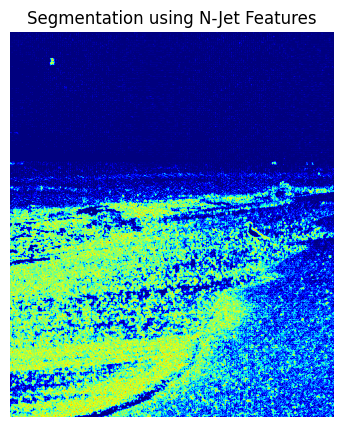
\includegraphics[width=\textwidth]{pics/a6-3.3-1.png}
        \caption{Segmentation using N-Jet Features}
        \label{fig:3.3-1}
    \end{minipage}
    \hfill
    \begin{minipage}{0.48\textwidth}
        \centering
        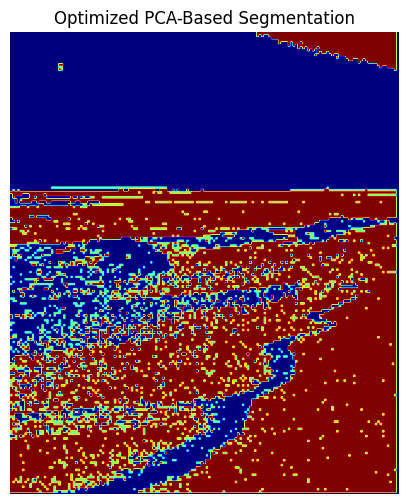
\includegraphics[width=\textwidth]{pics/a6-3.3-2.png}
        \caption{PCA-Based Segmentation}
        \label{fig:3.3-2}
    \end{minipage}
\end{figure}


The segmentation results shown in Fig \ref{3.3-1} and \ref{3.3-2} highlight the differences between the two approaches. The PCA-based segmentation method, which extracts local patches and applies dimensionality reduction before clustering, effectively captures broader image structures. It successfully differentiates large regions such as the sky, water, and landmass, leading to a more structured segmentation. However, since this method relies on patch-based feature extraction, some fine-grained textures may be lost, which affects the segmentation of detailed areas.

In contrast, the N-Jet-based segmentation with rotation invariance and PCA focuses on multi-scale edge and texture features. This approach enhances fine detail preservation, particularly in textured regions like the shoreline and water surface. The use of rotation invariance ensures that texture-based segmentation remains stable and consistent, even when patterns appear in different orientations. This makes the segmentation more robust to variations in the image structure.

Additionally, PCA plays a crucial role in both approaches by reducing the dimensionality of the feature space, which improves clustering performance and computational efficiency. Without PCA, the high-dimensional feature representation could lead to increased noise and make the clustering process less effective. Overall, the combination of N-Jet features with PCA results in segmentation that retains intricate texture details while maintaining efficiency in computation.


\end{document}
